\documentclass[es]{uc3mreport}

\usepackage{booktabs}

\usepackage{import}

\usepackage{mymacros}  % report-specific macros


% general config

\graphicspath{{img/}}  % Images folder
% \addbibresource{references.bib}  % bibliography file

\degree{Grado en Ingeniería Informática}
\subject{Inteligencia Artificial en las Organizaciones}
\year{2024-2025}  % academic year
\group{81}
\author{
    Álvaro Guerrero Espinosa -- 100472294 \\
    César López Mantecón -- 100472092 \\
    Paula Subías Serrano -- 100472119 \\
    Irene Subías Serrano -- 100472108
}
\team{Equipo 4}
\shortauthor{\abbreviateauthor{Álvaro}{Guerrero Espinosa}
             \abbreviateauthor{César}{López Mantecón}
             \abbreviateauthor{Paula}{Subías Serrano}
             \abbreviateauthor{Irene}{Subías Serrano}}
\lab{Práctica 2}
\title{Data Mining}
% \shorttitle{La mejor memoria de la historia}
\professor{Agapito Ledezma Espino}


\begin{document}
  \makecover[new]

  \tableofcontents
  \listoffigures
  \listoftables

  % contenidos
  \begin{report}

\section{Introducción}
\label{chap:intro}
En este documento se recoge el desarrollo de la segunda práctica de la asignatura \textit{Inteligencia Artificial en las Organizaciones}. El objetivo será la predicción de la valoración que un sujeto dará a su experiencia volando con una aerolínea a partir de distintos campos incluídos en una valoración. Dos de estos campos se tratan de datos textuales. Todo el estudio se llevará a cabo en la herramienta \href{https://altair.com/altair-ai-studio}{Altair AI Studio}.

Se obtendrán 3 modelos siguiendo distintas aproximaciones para predecir la clase a la que pertenece una crítica de un cliente en una aerolínea. Las estrategias a seguir son las siguientes: 

\begin{itemize}
    \item Modelo básico: se construye un modelo eliminando todos los atributos textuales.
    \item Modelo de \textit{text mining I}: se construye un modelo con procesamiento de texto, pero sin emplear análisis de sentimientos.
    \item Modelo de \textit{text mining II}: se construye un modelo con procesamiento de texto y análisis de sentimientos. Además en este modelo se hará uso de bigramas y trigramas.
\end{itemize}

El uso de análisis textual puede resultar útil dado al tipo de problema que se pretende resolver, ya que entre los datos aparecen campos textuales no estructurados. Este tipo de datos no podrán ser utilizados por otros modelos de aprendizaje automático debido a que, por si mismos, no son capaces de reconocer patrones o información incluidos en los datos. Complementariamente, el uso de \textit{análisis de sentimientos} ayudará a la predicción ya que la variable objetivo depende fuertemente de la opinión del autor del autor de la valoración. Además, al construir varios modelos se podrá comparar el aporte del \textit{text mining} y \textit{análisis de sentimietos} frente al modelo básico sin campos textuales.

El número de pasajeros de avión a lo largo de los últimos 10 años ha crecido enormemente, haciendo imposible usar técnicas tradicionales para el añálisis de la gran cantidad de datos que se disponen. Si tomamos como referencia el año 2019, año previo a la pandemia del \textit{covid-19}, hubo $4.490$ millones de pasajeros~\cite{owd-passengers}. Aunque únicamente un pequeño porcentaje de ellos dejara una valoración de su experiencia, la cantidad de datos para procesar sobrepasaría la capacidad de cualquir mecanismo tradicional de análisis de datos. Es por esto que el uso de algoritmos de \textit{minería de datos} es crucial para optener rendimiento de la información en este ámbito.

Además, esta clase de modelos cuentan con multitud de aplicaciones en diversos campos: la detección temprana de problemas en los servicios, la creación de marketing dirigido, el desarrollo de algoritmos de respuestas automáticas o el análisis competitivo de compañías para destacar sus fortalezas y puntos flacos en el mercado.

\section{Análisis exploratorio de los datos (EDA)}
\label{chap:eda}
Se ha realizado un estudio de todos los datos con el objetivo de su entendimiento para determinar el uso y necesidad de los mismos. Este análisis se ha realizado a través de las herramientas de Rapid Miner Statistics~\cite{Statistics-RM} y Correlation-Matrix~\cite{Correlation-Matrix-RM}. Además, se han explorado únicamente los datos de entrenamiento para evitar problemas de \textit{data\_leak}. 

El \textit{dataset} cuenta con 13643 instancias de reseñas de vuelos. Para cada reseña se incluyen 19 atributos de distinta naturaleza: campos textuales, fechas, datos categóricos y datos numéricos. A continuación haremos un breve repaso por cada uno de los atributos, explorando su tipo, su significado y el número de valores faltantes.

\begin{itemize}
    \item \textbf{Airline Name:} representa el nombre de la aerolínea asociado al vuelo reseñado. Se trata de un atributo \textit{nominal}.
    \item \textbf{Aircraft:} representa el modelo de avión empleado en el vuelo reseñado. Se trata de un atributo \textit{nominal}.  
    \item \textbf{Cabin Staff Service:} puntuación numérica del 0 al 50 sobre el servicio del personal a bordo. Se trata de un atributo \textit{numérico}. Cabe destacar que los valores que toma son siempre múltiplos de 10.
    \item \textbf{Date Flown:} fecha en la que se realizó el vuelo.
    \item \textbf{Food \& Beverages:} puntuación numérica del 0 al 50 sobre el servicio de comida en el vuelo. Se trata de un atributo \textit{numérico}. Cabe destacar que los valores que toma son siempre múltiplos de 10. 
    \item \textbf{Ground Service:} puntuación numérica del 0 al 50 sobre el servicio en tierra. Se trata de un atributo \textit{numérico}. Cabe destacar que los valores que toma son siempre múltiplos de 10.
    \item \textbf{Inflight Entertainment:} puntuación numérica del 0 al 50 sobre el servicio de entretenimiento durante el vuelo. Se trata de un atributo \textit{numérico}. Cabe destacar que los valores que toma son siempre múltiplos de 10.
    \item \textbf{Overall Rating:} puntuación numérica del 1 al 9. Representa el grado de satisfacción del cliente. Se trata de un atributo \textit{numérico}. Además, se trata de nuestra \textbf{variable objetivo}.
    \item \textbf{Recomended:} valor \textit{booleano}. Representa si el cliente recomendaría el servicio. Destaca un desbalanceo del 69.95\% hacia el valor negativo.
    \item \textbf{Review:} atributo \textit{textual}. Contiene el comentario del usuario sobre el vuelo.
    \item \textbf{Review Date:} fecha en la que se realizó la reseña.
    \item \textbf{Review Title:} campo \textit{texual}. Da título a la reseña. 
    \item \textbf{Route:} campo \textit{textual}. Representa la ruta del vuelo.
    \item \textbf{Seat Comfort:} puntuación numérica del 0 al 50 sobre la comodidad de los asientos. Se trata de un atributo \textit{numérico}. Cabe destacar que los valores que toma son siempre múltiplos de 10.
    \item \textbf{Seat Type:} atributo \textit{nominal}. Describe el tipo de asiento. Puede tomar los valores ``Ecoclass'',  ``Business Class'', ``Premium Economy'' y ``First Class''.  
    \item \textbf{Type Of Traveller:} atributo \textit{nominal}. Representa el tipo de viajero. Puede tomar los valores ``Solo Leisure'', ``Couple Leisure'', ``Family Leisure'' y ``Business''.
    \item \textbf{Value For Money:} puntuación numérica del 0 al 50 sobre el valor percibido con respecto al dinero gastado. Se trata de un atributo \textit{numérico}. Cabe destacar que los valores que toma son siempre múltiplos de 10.
    \item \textbf{Verified:} atributo \textit{booleano}. Representa si la persona que realiza la reseña está verificada. Ambas clases están balanceadas, con un 55.77\% de inclinación hacia la clase mayoritaria.
    \item \textbf{Wifi \& Connectivity:} puntuación numérica del 0 al 50 sobre la conexión a internet durante el vuelo. Se trata de un atributo \textit{numérico}. Cabe destacar que los valores que toma son siempre múltiplos de 10.
\end{itemize}
En la siguientes tablas se recogen los datos relevantes para cada atributo: 
\begin{table}[H]
    \center
    \begin{tabular}{@{}ccccc@{}}
        \toprule
        Atributo & Airline Name       & Aircraft & Cabin Staff Service & Date Flown \\ 
        \midrule
        Tipo     & Nominal            & Nominal  & Numérico            & Fecha      \\ 
        Min      & -                  & -        & 0                   & 04/01/2012 \\ 
        Max      & -                  & -        & 50                  & 07/01/2023 \\ 
        Media    & -                  & -        & 26.259              & -          \\ 
        Moda     & Tiger Air Australia& A320     & 10                  & 05/01/2023 \\ 
        missing (\%) & 0              & 70.57\%  & 16.81\%             & 11.82\%    \\ 
        \bottomrule
    \end{tabular} 
    \caption{Datos de los atributos - 1}
\end{table}

\begin{table}[H]
    \center
    \begin{tabular}{@{}cccc@{}}
        \toprule
        Atributo     & Food \& Beverages & Ground service & Inflight Entertainment \\ 
        \midrule
        Tipo         & Numérico          & Numérico       & Numérico               \\ 
        Min          & 0                 & 10             & 0                      \\ 
        Max          & 50                & 50             & 50                     \\ 
        Media        & 23.298            & 20.646         & 19.792                 \\ 
        Moda         & 10                & 10             & 10                     \\ 
        missing (\%) & 38.15\%           & 17.32\%        & 53.10\%                \\ 
        \bottomrule
    \end{tabular} 
    \caption{Datos de los atributos - 2}
\end{table}
\begin{table}[H]
    \center
    \begin{tabular}{@{}cccccc@{}}
        \toprule
        Atributo     & Overall Rating  & Recommended & Review  & Review Date & Review Title \\ 
        \midrule                      
        Tipo         & Numérico        & Booleano    & Textual & Fecha       & Textual      \\ 
        Min          & 1               & -           & -       & 22/11/2003  & -            \\ 
        Max          & 9               & -           & -       & 27/07/2023  & -            \\ 
        Media        & 3.368           & -           & -       &             & -            \\ 
        Moda         & 1               & NO          & -       & 16/07/2023  & -            \\ 
        missing (\%) & 0\%             & 0\%         & 0\%     & 0\%         & 0\%          \\ 
        \bottomrule
    \end{tabular} 
    \caption{Datos de los atributos - 3}
\end{table}
\begin{table}[H]
    \center
    \begin{tabular}{@{}ccccc@{}}
        \toprule
        Atributo     & Route               & Seat Confort & Seat Type     & Type of Traveller \\ 
        \midrule
        Tipo         & Nominal             & Numérico     & Nominal       & Nominal           \\ 
        Min          & -                   & 0            & -             & -                 \\ 
        Max          & -                   & 50           & -             & -                 \\ 
        Media        & -                   & 23.831       & -             &                   \\ 
        Moda         & Melbourne to Sydney & 10           & Economy Class & Solo Leisure      \\ 
        missing (\%) & 12.22\%             & 16.28\%      & 1.71\%        & 11.79\%           \\ 
        \bottomrule
    \end{tabular} 
    \caption{Datos de los atributos - 4}
\end{table}
\begin{table}[H]
    \center
    \begin{tabular}{@{}ccccc@{}}
        \toprule
        Atributo     & Value For Money & Verified  & Wifi \& Connectivity \\ 
        \midrule
        Tipo         & Numérico        & Booleano  & Numérico             \\ 
        Min          & 0               & -         & 10                   \\ 
        Max          & 50              & -         & 50                   \\ 
        Media        & 22.050          & -         & 15.228               \\ 
        Moda         & 10              & Verdadero & 10                   \\ 
        missing (\%) & 1.62\%          & 0\%       & 72.69\%              \\ 
        \bottomrule
    \end{tabular} 
    \caption{Datos de los atributos - 5}
\end{table}

\section{Preprocesado}
\label{chap:preprocess}
En este capítulo se describen las diferentes transformaciones aplicadas a los datos para su posterior uso en el entrenamiento de modelos.

\subsection{Transformación de \textit{OVERALL\_RATING} a nominal}
\label{sec:overalltransform}
Para poder construir un clasificador hemos transformado este atributo de numérico a nominal con 3 clases.
\begin{itemize}
    \item 1: agrupa los valores comprendidos entre 1 y 3, ambos incluídos.
    \item 2: agrupa los valores comprendidos entre 4 y 6, ambos incluídos.
    \item 3: agrupo los valores comprendidos entre 7 y 9, ambos incluídos.
\end{itemize}

De esta forma tambión logramos corregir la poca representación de algunos valores en el conjunto de datos. Cabe destacar que aun agrupando sigue habiendo una representación muy pobre de la clase \textit{2}.

\begin{table}[H]
    \begin{center}
        \begin{tabular}{@{}ccccc@{}}
            \toprule
            Clase                & 1              & 2      & 3\\ 
            \midrule
            Número de instancias & 8921           & 1148   & 3574 \\ 
            Porcentaje           & 65.39\%        & 8.41\% & 26.20\\ 
            \bottomrule
        \end{tabular} 
        \caption{Porcentaje de representación de cada clase}
    \end{center}
\end{table}

La sobrerrepresentación de la clase correspondiente a las evaluaciones más bajas se puede explicar a través de la tendencia de las personas a publicar una crítica en caso de descontento. A continuación se muestra un gráfico de tarta con la distribución de cada una de las clases:

\begin{figure}[H]
    \center
    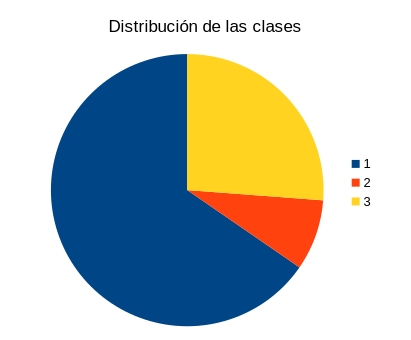
\includegraphics[width=0.60\linewidth]{overall_clases.png}\\ 
    \caption{Distribución de las clases}
\end{figure}

\subsection{Eliminación de atributos}
\label{sec:delete_columns}
Se han seguido 3 criterios para la eliminación de atributos:
\begin{itemize}
    \item Relevancia: algunos datos no aportan información relevante de cara al entrenamiento del modelo. Por este criterio se han eliminado \textit{Date Flown} y \textit{Date Review}.
    \item Afectar negativamente al modelo: algunos atributos nominales cuentan con un número de clases muy numeroso. En el caso de \textit{Route}, tratar con todas ellas añade una gran complejidad que no se traduce a un mejor rendimiento. En consecuencia, se ha eliminado este atributo. 
    \item Numerosos valores faltantes: se han eliminado todos los atributos con un número de \textit{missing values} superior al 35\% de los valores totales. Esto es porque se considera que no contamos con información suficiente para imputar estos datos.
\end{itemize}
A continuación se muestra un gráfico con el número de valores faltantes por atributo:

\begin{figure}[H]
    \center
    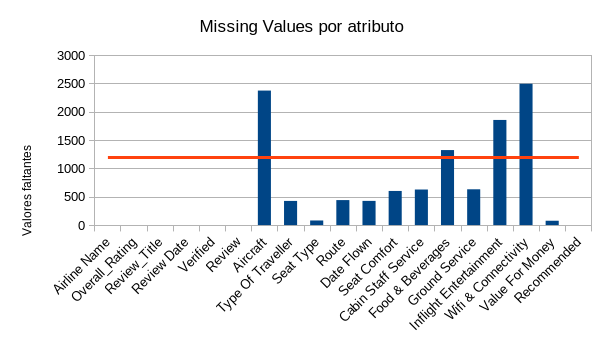
\includegraphics[width=0.85\linewidth]{missings.png}\\ 
    \caption{Número de valores faltantes por atributo}
\end{figure}

La línea sobre el gráfico señala el 35\% de las instancias. Por lo tanto, toda barra que rebase la línea se corresponde con un atributo a eliminar. Los atributos afectados han sido: \textit{Aircraft, Food \& Beverages, Inglight Entertainment} y \textit{Wifi \& Connectivity}.

\subsection{Formateo de los datos}
\label{sec:formateo}
Se han sustituído los valores de las columnas booleanas (i.e. \textit{Verified} y \textit{Recommended}) por valores binarios. Los valores nominales se han codificado mediante \textit{One-hot encoding}, a excepción de \textit{Airline} (esto es por limitaciones de la implementación). Los atributos codificados a través de \textit{OHE} han sido \textit{Seat Type} y \textit{Type of Traveller}.

\subsection{Imputación de valores faltantes}
\label{sec:imputacion}
En cuanto a la imputación de valores faltantes, se han reemplazado mediante el operador \textit{Replace Missing Values} de \textit{Altair AI Studio} por la moda de cada atributo. Los atributos afectados han sido \textit{Type Of Traveller, Seat Type, Food \& Bervarges, Groud Service, Seat Confort} y \textit{Value For Money}.

\section{Modelo básico sin usar datos textuales}
\label{chap:basicModel}
Se ha entrenado un modelo básico utilizando \textit{deep learning} para utilizarlo como referencia y cuantificar los beneficios proveídos por el \textit{text mining}. En la fase de preprocesado de los datos de este modelo solo se realiza la limpieza de datos relacionada con reemplazar datos faltantes y seleccionar atributos, eliminando todos los atributos de texto.

Se ha entrenado un modelo básico de \textit{deep learning} para utilizarlo como referencia y cuantificar los beneficios proveídos % paula en su momento de máxima inspiración lírica fdo. César
por el \textit{text mining}. Además del preprocesado de los datos especificado anteriormente, se han eliminando los atrbutos textuales \textit{Review} y \textit{Review Title}.

Tanto en el proceso de entrenamiento como en la evaluación se observa una \textit{accuracy} aproximada del 91\%. Se puede observar en la matriz de confusión que los resultados tanto de \textit{precission} como de \textit{recall} son muy buenos para las clases 1 y 3, siendo los valores en ambos casos cercanos al 90\%. Sin embargo, en el caso de la clase 2, estos los valores no alcanzan el 50\% de \textit{precission}. Concluímos que esto se debe a la poca representación de los datos de esta clase (8\%).

\section{Proceso de entrenamiento}
\label{chap:train}

\subsection{Parte 1 - Modelado sin análisis de sentimientos}
\label{sec:parte1}

    Para el entrenamiento de distintos modelos trabajaremos con variaciones
    sobre los parámetros del preprocesado de los datos y los modelos usados.
    Además, hemos empleado distintos tipos de modelo con sus
    parámetros por defecto con el fin de tener una mayor variedad y encontrar
    el más efectivo.

    Cabe destacar que también se ha intentado usar ``Support Vector Machine'',
    pero no se ha podido ya que no soporta los atributos de tipo polinómico.

    De esta forma, estamos empleando un \textit{grid-search} con los siguientes valores:
    \begin{itemize}
        \item Preprocesado: \{\textit{TF-IDF}, \textit{Binary Term Occurrence}, \textit{prune below $10\%$}\}.
        \item Modelos: \{\textit{Deep Learning}, \textit{Random Forest}, \textit{Naive Bayes}, \textit{Decision Trees}\}
    \end{itemize}

    Al concluir el entrenamiento hemos obtenido los siguientes resultados:

    \footnotetext[1]{El formato de los parámetros es el siguiente: (\textit{Vector creation}, porcentaje de \textit{prune below}, modelo usado)}
    \begin{table}[H]
        \begin{center}
            \begin{tabular}{ @{}clc@{} }
                \toprule
                Modelo & Parámetros\footnotemark[1] & Accuracy\\
                \midrule
                1  & (\textit{TF-IDF}, $3\%$                 \textit{Deep Learning})  & 0.891\\
                2  & (\textit{TF-IDF}, $3\%$                 \textit{Random Forest})  & 0.848\\
                3  & (\textit{TF-IDF}, $3\%$                 \textit{Naive Bayes})    & 0.790\\
                4  & (\textit{TF-IDF}, $3\%$                 \textit{Decision Trees}) & 0.866\\
                5  & (\textit{Binary Term Occurrence}, $3\%$ \textit{Deep Learning})  & 0.898\\
                6  & (\textit{Binary Term Occurrence}, $3\%$ \textit{Random Forest})  & 0.882\\
                7  & (\textit{Binary Term Occurrence}, $3\%$ \textit{Naive Bayes})    & 0.772\\
                8  & (\textit{Binary Term Occurrence}, $3\%$ \textit{Decision Trees}) & 0.887\\
                9  & (\textit{TF-IDF}, $10\%$,               \textit{Deep Learning})  & 0.899\\
                10 & (\textit{TF-IDF}, $10\%$,               \textit{Random Forest})  & 0.890\\
                11 & (\textit{TF-IDF}, $10\%$,               \textit{Naive Bayes})    & 0.794\\
                12 & (\textit{TF-IDF}, $10\%$,               \textit{Decision Trees}) & 0.867\\
                \bottomrule
            \end{tabular}
            \caption{Errores de los diferentes modelos - Parte 1}
        \end{center}
    \end{table}

    Si observamos la comparación por pares proporcionada por el \textit{t-test},
    destaca el modelo 9 por obtener los mejores resultados y ser significativamente
    diferente de todos los demás modelos excepto uno. A continuación se muestra
    la matriz resultante de la ejecución del test:

    \begin{figure}[H]
        \center
        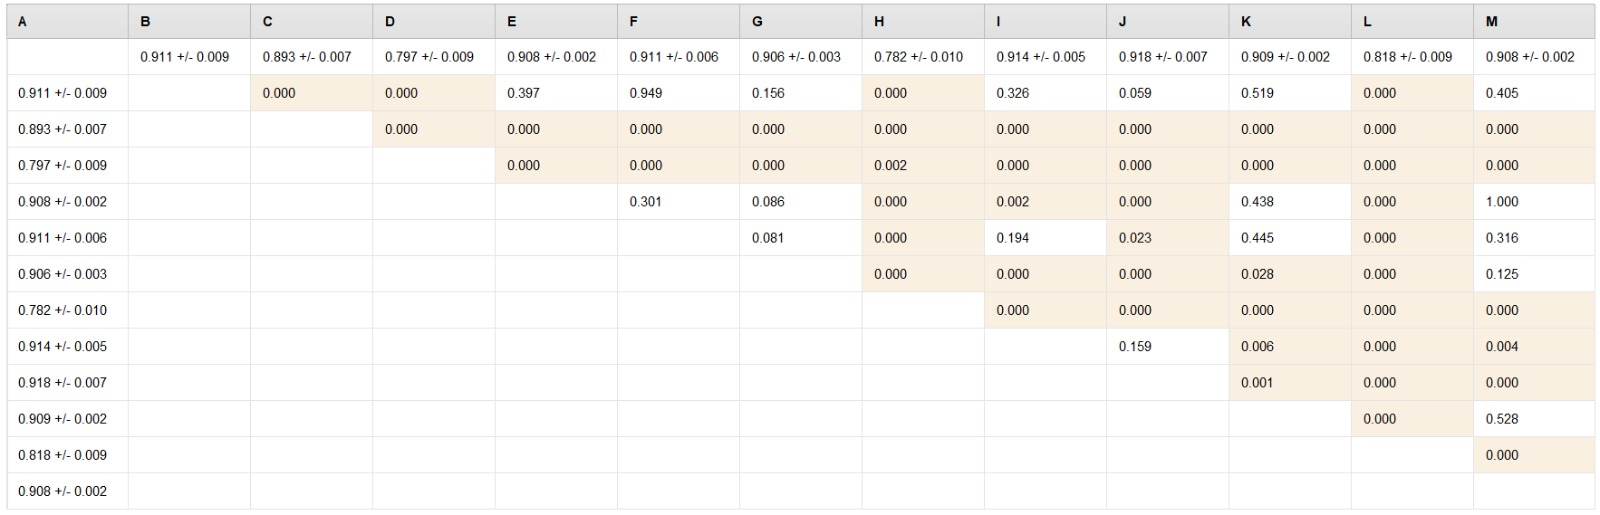
\includegraphics[width=\linewidth]{t_test1.jpeg}\\ 
        \caption{Resultados de los modelos en el conjunto de \textit{train} - Parte 1}
    \end{figure}

    Con toda esta información concluimos que el mejor modelo y con el que haremos
    la predicción es el modelo 9, debido a que es el modelo con mejor
    \textit{accuracy} y es de los modelos más simples al usar \textit{prune below $10\%$}.
    En la siguiente figura se muestra el \textit{recall} y \textit{precision}
    de las diferentes clases para este modelo.

    \begin{figure}[H]
        \center
        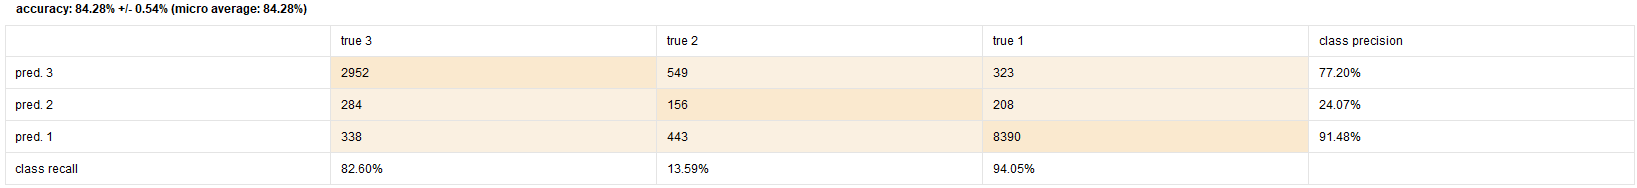
\includegraphics[width=\linewidth]{train1.jpeg}\\ 
        \caption{Errores del modelo 9 en el conjunto de \textit{train} - Parte 1}
    \end{figure}

\subsection{Parte 2 - Modelado con análisis de sentimientos}
\label{sec:parte2}

    Al igual que en la parte anterior, trabajaremos con variaciones
    sobre los parámetros del preprocesado de los datos y los modelos usados.

    De esta forma estamos empleando un \textit{grid-search} con los siguientes valores:
    \begin{itemize}
        \item Preprocesado: \{\textit{bigramas}, \textit{trigramas}, \textit{prune below $10\%$}\}.
        \item Modelos: \{\textit{Deep Learning}, \textit{Random Forest}, \textit{Naive Bayes}, \textit{Decision Trees}\}
    \end{itemize}

    Al concluir el entrenamiento hemos obtenido los siguientes resultados:

    \footnotetext[2]{El formato de los parámetros es el siguiente: (Longitud $n$-gramas, porcentaje de \textit{prune below}, modelo usado)}
    \begin{table}[H]
        \begin{center}
            \begin{tabular}{ @{}clc@{} }
                \toprule
                Modelo & Parámetros\footnotemark[2] & Accuracy\\
                \midrule
                1  & (\textit{Bigramas},  $3\%$, \textit{Deep Learning})  & 0.905\\
                2  & (\textit{Bigramas},  $3\%$, \textit{Random Forest})  & 0.887\\
                3  & (\textit{Bigramas},  $3\%$, \textit{Naive Bayes})    & 0.797\\
                4  & (\textit{Bigramas},  $3\%$, \textit{Decision Trees}) & 0.909\\
                5  & (\textit{Trigramas}, $3\%$, \textit{Deep Learning})  & 0.902\\
                6  & (\textit{Trigramas}, $3\%$, \textit{Random Forest})  & 0.884\\
                7  & (\textit{Trigramas}, $3\%$, \textit{Naive Bayes})    & 0.797\\
                8  & (\textit{Trigramas}, $3\%$, \textit{Decision Trees}) & 0.909\\
                9  & (\textit{Bigramas}, $10\%$, \textit{Deep Learning})  & 0.919\\
                10 & (\textit{Bigramas}, $10\%$, \textit{Random Forest})  & 0.909\\
                11 & (\textit{Bigramas}, $10\%$, \textit{Naive Bayes})    & 0.819\\
                12 & (\textit{Bigramas}, $10\%$, \textit{Decision Trees}) & 0.909\\
                \bottomrule
            \end{tabular}
            \caption{Errores de los diferentes modelos - Parte 2}
        \end{center}
    \end{table}

    Al igual que en la parte anterior, si observamos la comparación por pares
    proporcionada por el \textit{t-test}, destaca el modelo 9 (\textit{Deep Learning}
    con \textit{prune below $10\%$}). A continuación se muestra la matriz resultante
    de la ejecución del test:

    \begin{figure}[H]
        \center
        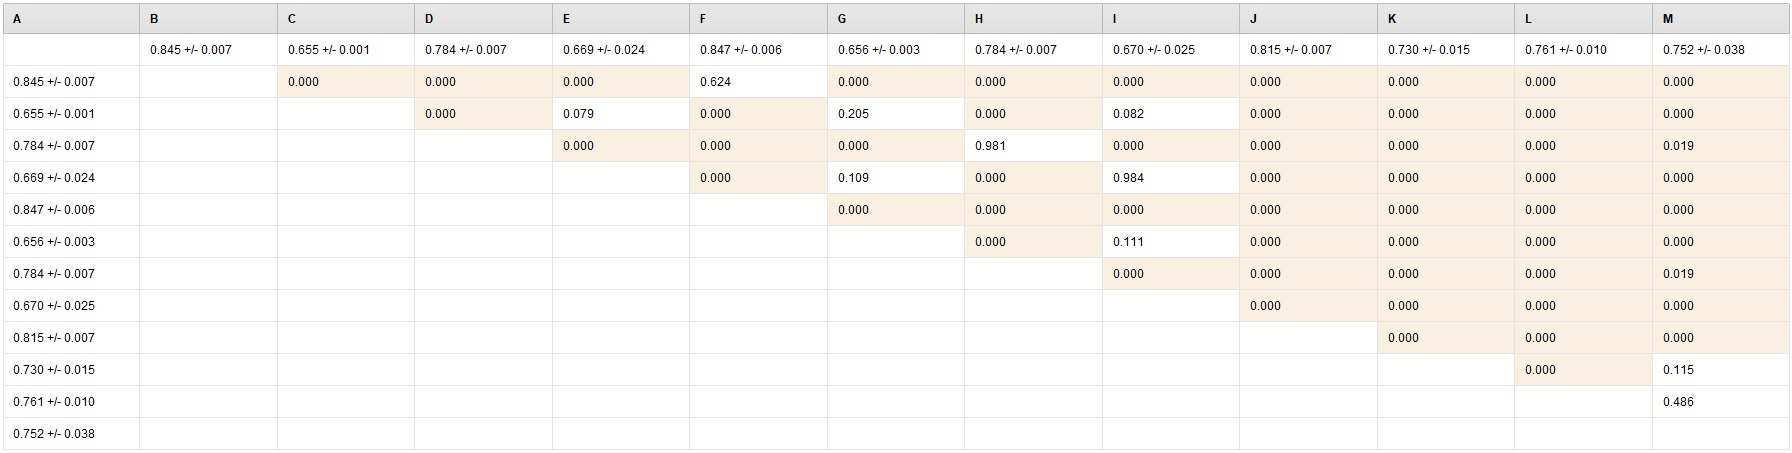
\includegraphics[width=\linewidth]{t_test2.jpg}\\ 
        \caption{Resultados de los modelos en el conjunto de \textit{train} - Parte 2}
    \end{figure}

    Con toda esta información concluimos que el mejor modelo y con el que haremos
    la predicción es el modelo 9, debido a que es el modelo con mejor
    \textit{accuracy} y es de los modelos más simples al usar \textit{bigramas}
    con \textit{prune below $10\%$}. En la siguiente figura se muestra el 
    \textit{recall} y \textit{precision} de las diferentes clases para este modelo.

    \begin{figure}[H]
        \center
        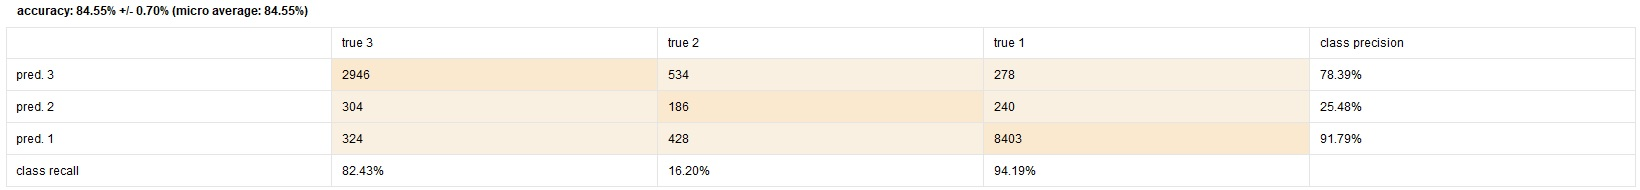
\includegraphics[width=\linewidth]{train2.jpeg}\\ 
        \caption{Errores del modelo 9 en el conjunto de \textit{train} - Parte 2}
    \end{figure}

\section{Comparación de resultados}
\label{chap:resultados}

\section{Conclusión}
\label{chap:conclusion}

Esta práctica nos ha permitido explorar nuevas técnicas para la construcción de modelos. En concreto, hemos podido comprobar como el \textit{text mining} presenta grandes ventajas frente a modelos que no aprovechan toda la información contenida en campos de texto.

Además, el análisis de sentimientos ha demostrado ser de gran utilidad en esta clase de aplicaciones. Conocer el sentimiento de un agente hacia un dominio mediante el análisis de datos tiene muy buenas aplicaciones en el campo del marketing y el análisis empresarial.

  \end{report}


  % bibliography
  \label{bibliography}
  \part{Bibliografía}
  \printbibliography
  % % \printbibliography[title={Referencias}]  % alternative

  % appendices
  % \begin{appendices}
  %   \part{Apéndices}  % optional
  %   \section{Mi apéndice}
  %   \lipsum[1]
  % \end{appendices}

\end{document}
